\documentclass[12pt]{article}
\usepackage[margin=0.5in]{geometry}
\usepackage{graphicx}
\usepackage{amsmath}
\usepackage{subcaption}
\usepackage{float}
\pagestyle{headings}
\begin{document}
\begin{center}
{\LARGE \textbf{City Clustering From Road Network Graph}}
\end{center}
\begin{center}
Wenjian Hu, Jian Xu
\end{center}
\begin{center}
{\Large \textbf{1. Background}}
\end{center}
\textbf{1.1 Introduction} The efficient plan and development of cities has become an important topic nowadays. Data of city are collected from different means including GPS, mobile phone and user-generated media. Urban geographers, economists and tech companies have been using these data, along with computing and analysis tools to study and make orderly city development plans.
 
Road graph network is one significant source of region data. It can improve traffic condition. In the taxi study, the travel time and speed can be predicted. Also, road pattern can be identified, which helps to find hotspot locations and detect the anomalities over time. Taxi drivers can utilize the information to categorize taxi pick-up and drop-off region in more accurate smaller units [1]. Also, road graph is the base of social road sharing problem. Companies like Uber and Lyft allows users to share their positions and arrange route sharing. Bistaffa et al. developed a coalition formation algorithm, which resulted in a $36.22\%$ cost reduction from a 100-agent size system [2,3]. 
 
Road graph is a good source to study the urban distribution. For this purpose, cluster identification becomes very useful. Homogeneous regions in spatial data can be identified from cluster study. Different size of cluster may correspond to different functional units. A summary of the cluster data may provide a new perspective for future planning of city development [4]. Also, the real world geographical information can be further used to develop the cities’ social economic indicator and track urban land use [5]. Shan Jiang et al. incorporate time dimension into the spatial data. Human activity patterns like phone usage are traced and studied. Individuals are clustered according to their daily activity pattern with spatial-temporal traces. As a result, the activities of different type of individuals are visualized in the time-cumulative spatial density, and will be crucial for city function region design [6]. \\\\
\textbf{1.2 Methods.} Rather than using hierarchical clustering, we will use a quite different approach based from graph partitioning where a partition of the graph is determined by optimizing a merit function [7]. Defying intersections as nodes and the roads connecting these intersections as undirected edges (without edge weight information), we will deduce different clusters (cities) by calculating the conductance of different sets of nodes. A portion of PA road network data from SNAP database [8] will be used to build up our graph.

However, finding cuts with exactly minimal conductance is NP-hard, thus, we will use several algorithms with good approximation performance guarantees. First, we will apply the spectral method, which uses an eigenvector of the graph’s Laplacian matrix to find a cut whose conductance is no bigger than $\phi$ if the graph actually contains a cut with conductance $O(\phi2)$ [9,10,11]. Also, we will use max flow quotient cut improvement (MQI) method, which consists of random initial partition followed by a flow-based MQI post-processing [12,13]. \\\\
\textbf{1.3 Previous Work.} Very relevant to our work is that of Kannan, Vempala, and Vetta [14], who analyze spectral algorithms and describe a community concept in terms of a bicriterion depending on the conductance of the communities and the relative weight of inter-community edges. Flake, Tarjan, and Tsioutsiouliklis [15] introduce a similar bicriterion that is based on network flow ideas, and Flake et al. [16, 17] defined a community as a set of nodes that has more intra-edges than inter-edges. Similar edge-counting ideas were used by Radicchi et al. [18] to define and apply the notions of a strong community and a weak community.\\\\
\textbf{1.4 This Project.} In this project, we will be working on finding clusters (cities) from complicated road network graphs. We will approach the cut-improvement problem using the combination of spectral clustering method and MQI method, in contrast with the previous single method approach. In this project, the fundamental question we wish to answer is how to efficiently and accurately identify clusters from an undirected graph with multiple connected components.\\\\
\begin{center}
{\Large \textbf{2. Methods and Techniques}}
\end{center}
Hierarchical clustering is a common method of cluster analysis which seeks to build a hierarchy of clusters, in which procedure, one first need to define distances between pairs of nodes and then produces a tree describing how nodes group into communities and how these group further into super-communities. A quite different approach that has received a great deal of attention is based on
ideas from graph partitioning, in which case, the network is a module as simple undirected graph,
where nodes and edges have no attributes, and a partition of the graph is determined by optimizing a merit function. \\\\
\textbf{2.1 Definitions.}\\
\textit{\textbf{Definition 1} Given a graph $G = (V, E)$ with adjacency matrix  $W =(w_{ij})_{i,j=1,...,n}$ the conductance $\phi$ of a set of nodes $A\subset V$ is defined as:
$$\phi(A)=\frac{\sum_{i\in A,j\not\in A}w_{ij}}{min\{Vol\{A\},Vol\{\bar{A}\}\}}$$
where $Vol(A)=\sum_{i\in A}\sum_{j\in V}w_{ij}$, or equivalently $Vol(A)=\sum_{i\in A}d(i)$, where $d(i)$ is a degree of node i in G.}\\

Thus, the conductance of a set provides a measure for the quality of the cut $(A,\bar{A})$, or relatedly the goodness of a community $A$. Let $Vol(A)$ be the sum of degrees of nodes in $A$, and let $c$ be the number of edges with one endpoint in $A$ and one endpoint in $\bar{A}$, where $\bar{A}$ denotes the complement of $A$. Then, equivalently the conductance of $A$ is $\phi(A)= \frac{c}{Vol(A)}$.

In order to more finely resolve community structure in large networks, we introduce the network community profile plot (NCP plot). Intuitively, the NCP plot measures the quality of the best possible community in a large network, as a function of the community size. Formally, we may define it as the conductance value of the best conductance set of cardinality k in the entire network, as a function of k.

\begin{figure}[h]
\begin{center}
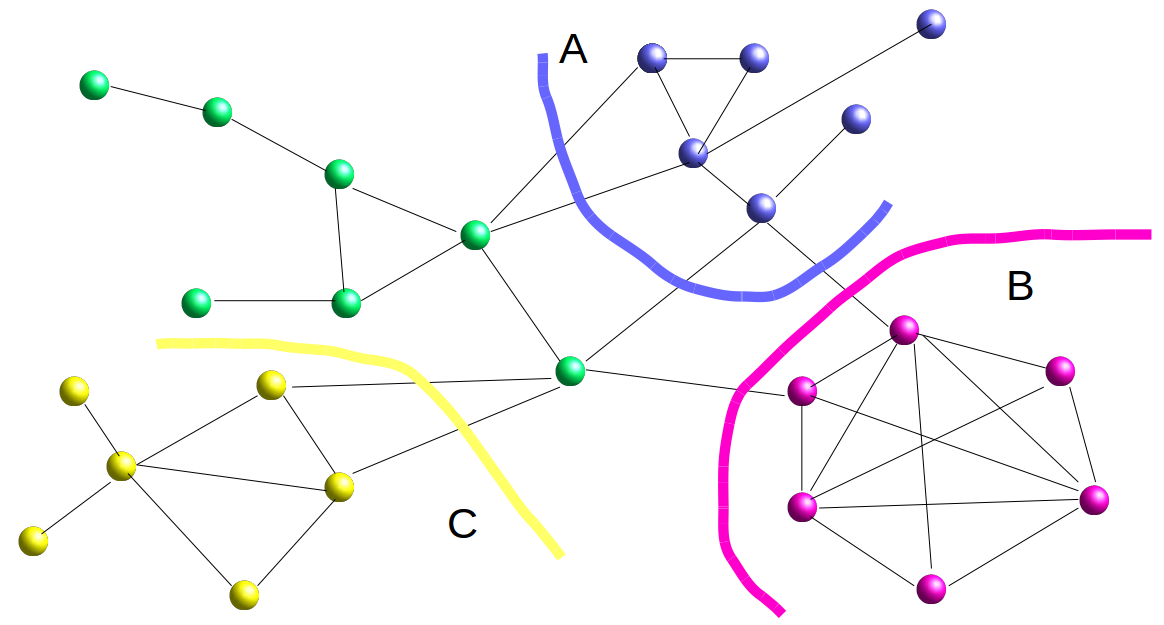
\includegraphics[scale=0.2]{network_clustering.png}  
\caption{Network communities. Of the three 6-nodes sets that have been marked, B has the best (i.e., the lowest) conductance, as it has the lowest ratio between the number of edges cut and the sum of degrees of nodes.}
\end{center}
\end{figure}

\textit{\textbf{Definion 2} Given a graph $G$ with adjacency matrix $W =(w_{ij})_{i,j=1,...,n}$, the network community profile plot (NCP plot) plots $\phi(k)$ as a function of $k$, where
$$\Phi(k)=min_{A \subset V, |A|=k}\phi(A)$$
where $|A|$ denotes the cardinality of the set $A$ and the conductance $\phi(A)$ of $A$ is given by definition 1.}\\

There are two main advantages about NCP plots [7]. First, minima in the NCP plots, i.e., the
best low-conductance cuts of a given size, correspond to communities-like sets of nodes. Second, the NCP plots are generally relatively gradually sloping downwards, meaning that smaller communities can be combined into larger sets of nodes that can also be meaningfully interpreted as communities.\\

However, finding cuts with exactly minimal conductance is NP-hard, thus, we are going to deal with this problem using several algorithms with provable approximation performance guarantees.\\\\
\textbf{2.2 Approximation Methods.}\\
\textbf{2.2.1 Spectral Clustering}[19]. Let $G = (V, E)$ be an undirected graph with vertex set $V = \{v_1 ,..., v_n \}$. In the following we assume that the graph $G$ is weighted, that is each edge between two vertices $v_i$ and $v_j$ carries a non-negative weight $w_{ij}\geq 0$. The weighted adjacency matrix of the graph is the matrix $W =(w_{ij})_{i,j=1,...,n}$. If $w_{ij}=0$ this means that the vertices $v_i$ and $v_j$ are not connected. As $G$ is undirected we require $w_{ij}= w_{ji}$. The degree of a vertex $v_i \in V$ is defined as
$$d_i=\sum^n_{j=1}w_{ij}$$

The degree matrix $D$ is defined as the diagonal matrix with the degrees $d_1 ,..., d_n$ on the diagonal. Given a subset of vertices $A \subset V $, we denote its complement $V-A$ by $\bar{A}$. For convenience, we introduce the shorthand notation $i \in A$ for the set of indices $\{i| v_i \in A\}$. We consider two different ways of measuring the “size” of a subset $A \subset V$ :
\begin{center}
$|A|$:= the number of vertices in $A$\\
$vol(A):=\sum_{i \in A}d_i$
\end{center}

A subset $A \subset V$ of a graph is connected if any two vertices in $A$ can be joined by a path such that all intermediate points also lie in $A$. A subset $A$ is called a connected component if it is connected and if there are no connections between vertices in $A$ and $\bar{A}$. The sets $A_1 ,..., A_k$ form a partition of the graph if $A_i \cap A_j =\emptyset$ and $A_1 \cup...\cup A_k = V$. \\

The unnormalized graph Laplacian matrix is defined as
$$L=D-W$$

Then we can compute the first $k$ eigenvectors $v_1 , . . . , v_k$ of $L$. Let $V$
be the matrix containing the vectors $v_1 , . . . , v_k$ as columns. For $i=1, . . . ,n,$ let $y_i$ be the vector corresponding to the ith row of V . Cluster the points $(y_i)_{i=1,...,n}$ with the k-means algorithm into clusters $C_1 , . . . , C_k$ and output clusters $A_1 , . . . , A_k$ with $A_i = \{ j | y_j \in C_i \}$. Through this method, we will be able to identity connected components in a complicated graph, just by setting the cluster number equal the multiplicity of the eigenvalue $0$ of $L$. Formally, we have the following proposition:\\\\
\textit{\textbf{Proposition 1 (Number of connected components)} Let $G$ be an undirected graph with non-negative weights. Then the multiplicity $k$ of the eigenvalue $0$ of $L$ equals the number of connected components $A_1 ,..., A_k$ in the graph. The eigenspace of eigenvalue $0$ is spanned by the indicator vectors $\vec{1}_{A_1} ,...,\vec{1}_{A_k}$ of those components, where the indicator vector $\vec{1}_A = (f_1 ,..., f_n) \in R^n$ as the vector with entries $f_i = 1$ if $v_i \in A$ and $f_i = 0$ otherwise.}\\\\
\textbf{2.2.2 Max Flow Quotient Cut Improvement (MQI)}[20].
For this technique, our input is an undirected graph and an initial cut, that is, an initial partitioning of the graph’s nodes into two sets $A$ and $B = \bar{A}$. WLOG $Vol(A) \leq Vol(B)$. There are $c$ edges crossing the cut, so the initial quotient cut score (conductance) is $c/Vol(A)$. Figure 2 is a schematic diagram of the flow problem that we will build. \\
\begin{figure}[h]
\begin{center}
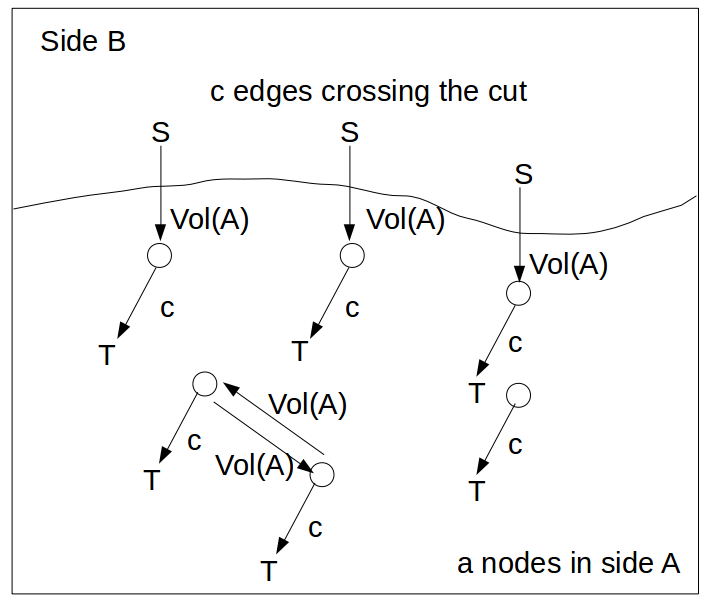
\includegraphics[scale=0.38]{MQI.png}  
\caption{Setting up the max flow problem.}
\end{center}
\end{figure}

Note that although this problem will be based on our undirected input graph and cut, we are building a completely new directed graph here. The algorithm is as follow:
\begin{enumerate}
\item Discard all $B$-side nodes.
\item Discard every edge that used to connect a pair of $B$-side nodes.
\item Replace every edge that used to connect a pair of $A$-side nodes with a pair
of directed edges, one pointing in each direction, and each with capacity $Vol(A)$.
\item Add a source node $S$ and a sink node $T$.
\item Discard each edge that used to connect a $B$-side node with an $A$-side node
x, replacing it with a single directed edge from $S$ to x, with capacity $Vol(A)$.
\item Add a single directed edge from every $A$-side node to $T$ , with capacity c.
\end{enumerate}
After we build up the above max flow problem, we need to find a solution to this max flow problem and then use this solution to build up the new partition $A'$ and $B'=\bar{A'}$ shown in Figure 3. First, here is a theorem we will use:\\\\
\textit{\textbf{Theorem 1}. There is an improved quotient cut $(A',B')$ (with $A'$ a strict subset
of $A$) if and only if the maximum flow is less than $ca$, where $a=|A|$.}\\\\
\begin{figure}[h]
\begin{center}
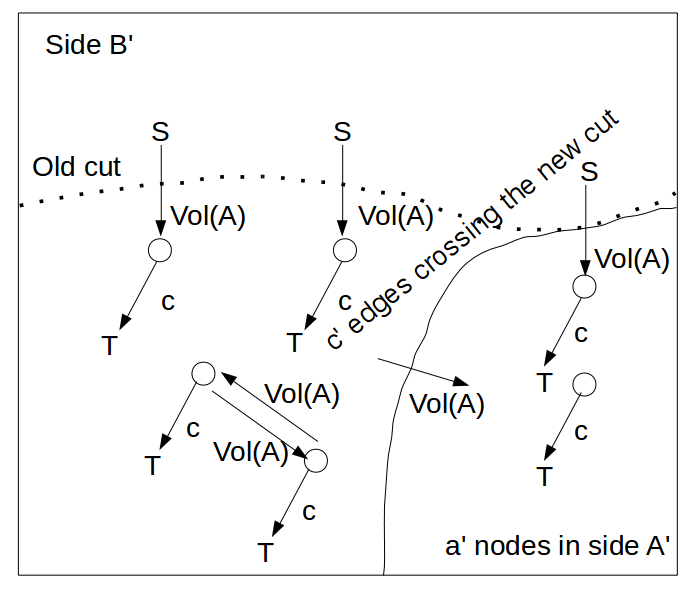
\includegraphics[scale=0.4]{MQI2.png}  
\caption{Interpreting the solution of the maximum flow problem and building up the new quotient cut $A',B'$.}
\end{center}
\end{figure}
In the new partition, the small side $A'$ is the set of nodes reachable from the sink by a depth-first search along reversed unsaturated edges. This “backwards DFS” procedure advances from a node y to a node x if and only if there is an unsaturated edge leading from node x to node y. The conductance of the new cut $A'$, $\frac{c'}{Vol(A')}$, is smaller than the conductance of the old cut $A$, $\frac{c}{Vol(A)}$. A single call to MQI determines whether any reachable improved quotient cut exists, and if so, it returns one of them. To find the minimum conductance cut, we simply perform multiple tries of MQI with different RNG seeds for the initial partition. \\
\begin{center}
{\Large \textbf{3. Main Algorithm (Plan)}}
\end{center}
So far, we have introduced our two main methods, spectral clustering method and max flow quotient cut improvement (MQI) method. In order to efficiently and accurately tackle undirected road graphs with multiple connected components, we combine these two methods and form our main algorithm as follow:
\begin{enumerate}
\item Load the data and form undirected graph $G$
\item Build up the adjacency matrix $W$ and degree matrix $D$. Since our input graph has no weight, we simply set each edge has the same weight $1$.
\item Build up the Laplacian matrix $L=D-W$.
\item Solve the Laplacian matrix $L$ and get corresponding eigenvalues and eigenvectors. Partition the original graph $G$ into k, which is the multiplicity of the eigenvalue $0$ of $L$, connected components $A_{1},A_{2},...,A_{k}$, so that each subset $A_i \subset G$ has no connections with $\bar{A_i}$.
\item For each subset $A_i \subset G$, repeatedly use random initial partition $+$ max flow quotient cut improvement method to collect data for NCP plot.
\item For each subset $A_i \subset G$, draw its NCP plot and conclude its best possible community in that subset from the minimum point in that NCP plot. 
\end{enumerate}
\begin{center}
{\Large \textbf{4. Results and Analysis}}
\end{center}
To see the importance of combining these two methods to deal with undirected multiple connected components graphs, we first demonstrate the results of only using MQI method in Figure 4:
\begin{figure}[h]
\begin{center}
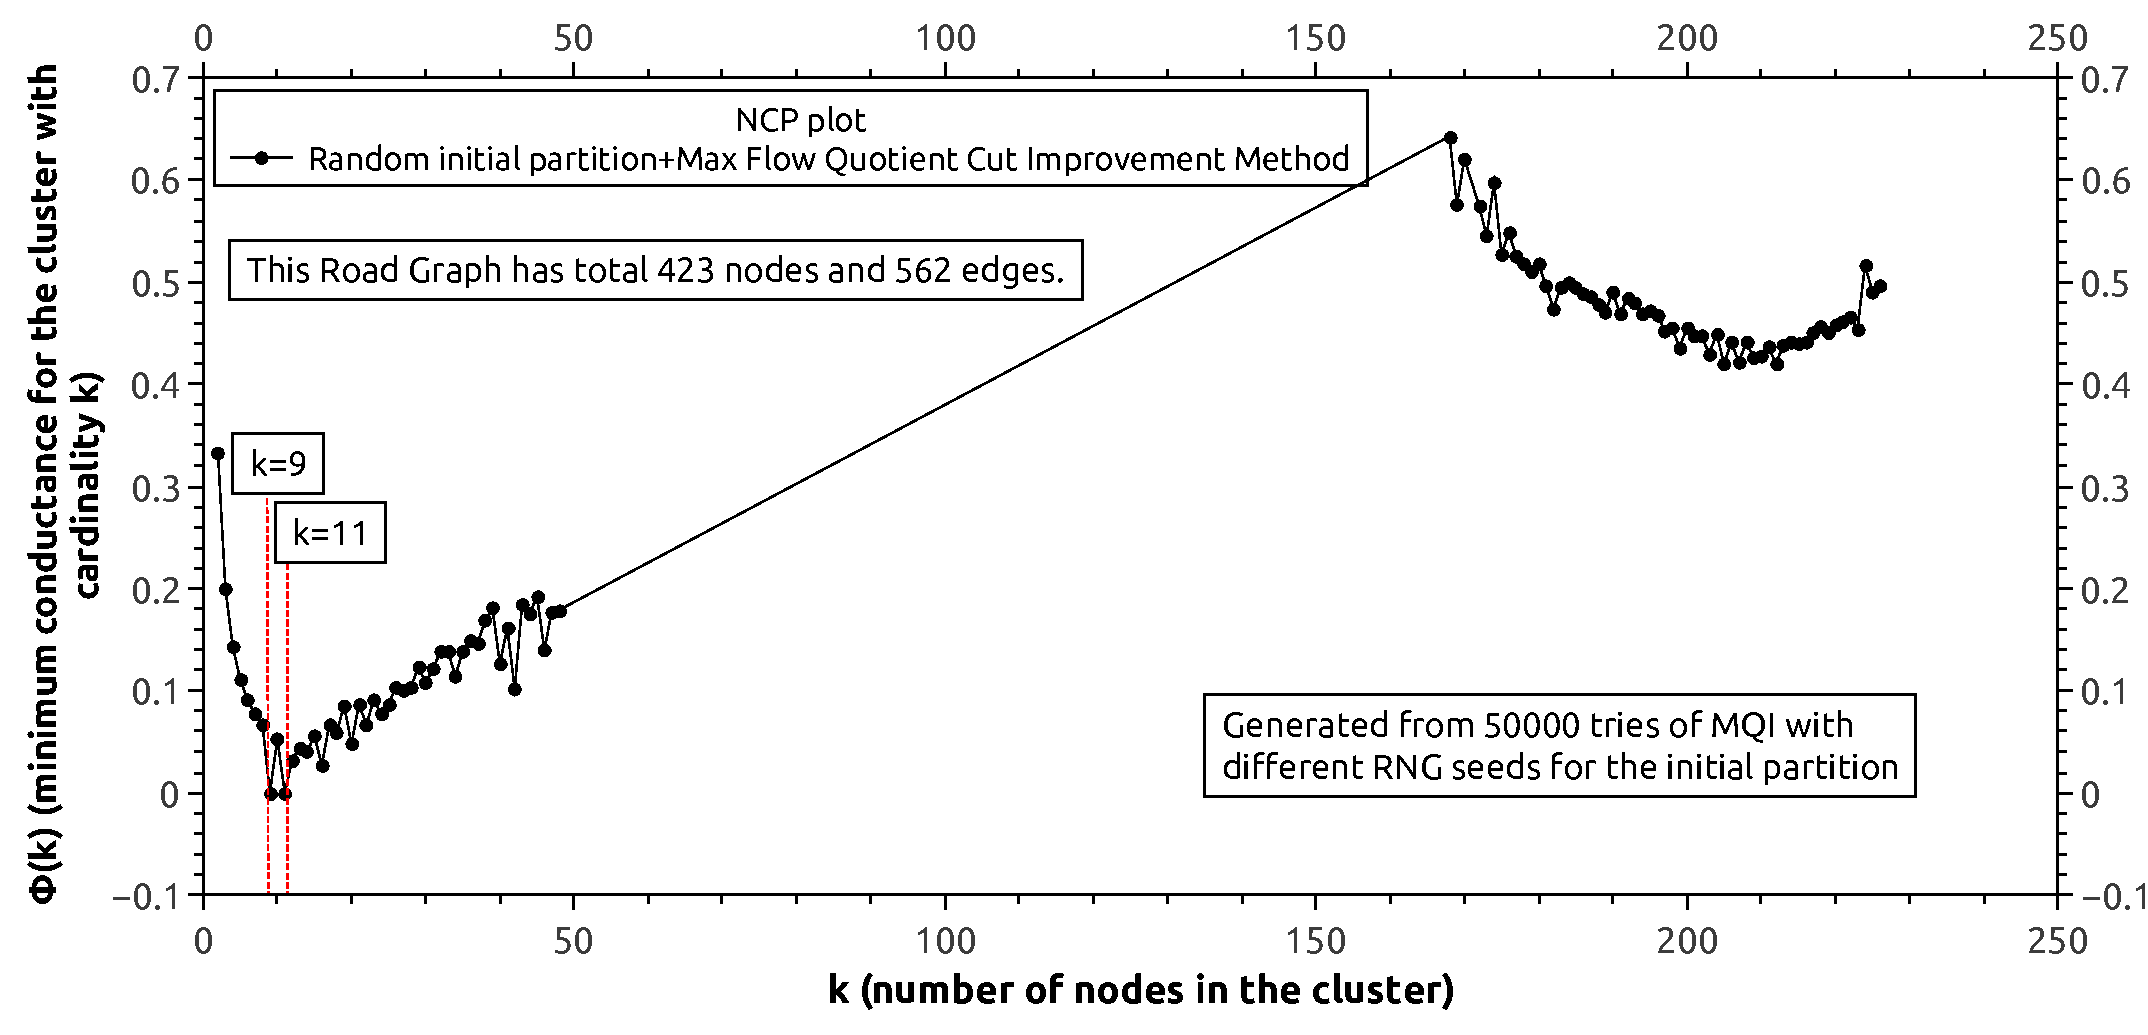
\includegraphics[scale=0.45]{MQI_only.pdf}
\caption{NCP plot only using MQI method}
\end{center}
\end{figure}

If a graph exists multiple connected components and a cut happens to be in between these connected components, the corresponding conductance of this cut is $0$, since there is no edges crossing different connected components. Figure 4 has two minima (zero) conductance cuts at size $k=9$ and $k=11$, which means the above road graph has at least two connected components with size $k=9$ and $k=11$. Usually, the minima in the NCP plots, i.e., the best low-conductance cuts of a given size, correspond to communities-like sets of nodes. Here, we find two connected components just by searching the minima in the above NCP plot, since zero conductance is always lowest if it exists and a single connected component is truly the most communities-like. 

However, we are still not sure how many connected components exist and we know nothing about the most communities-like set in each connected component, which is usually more concerned to us. Thus, to fully understand the cluster information in such graphs, we still need to further combine MQI method with spectral clustering method, which is usually very powerful to detect all the connected components. Here are the results of using both of them:\\
\begin{figure}[H]
  \begin{subfigure}[b]{0.5\textwidth}
    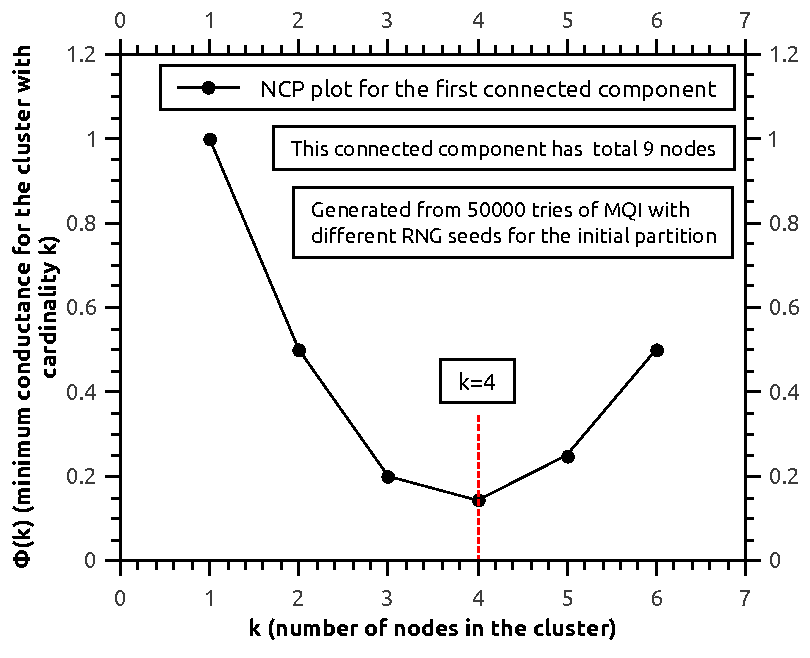
\includegraphics[scale=0.66]{MQI_1.pdf}     
    \label{fig:1}
  \end{subfigure}
  %
  \begin{subfigure}[b]{0.5\textwidth}
    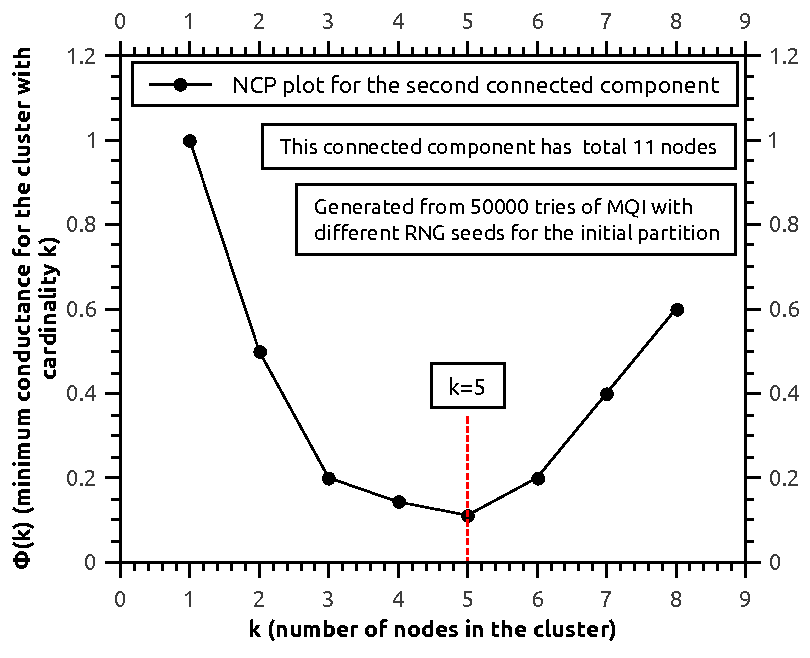
\includegraphics[scale=0.66]{MQI_2.pdf} 
    \label{fig:2}
  \end{subfigure}
  \caption{NCP plot of the first/second connected component}
\end{figure}
\begin{figure}[h]
\begin{center}
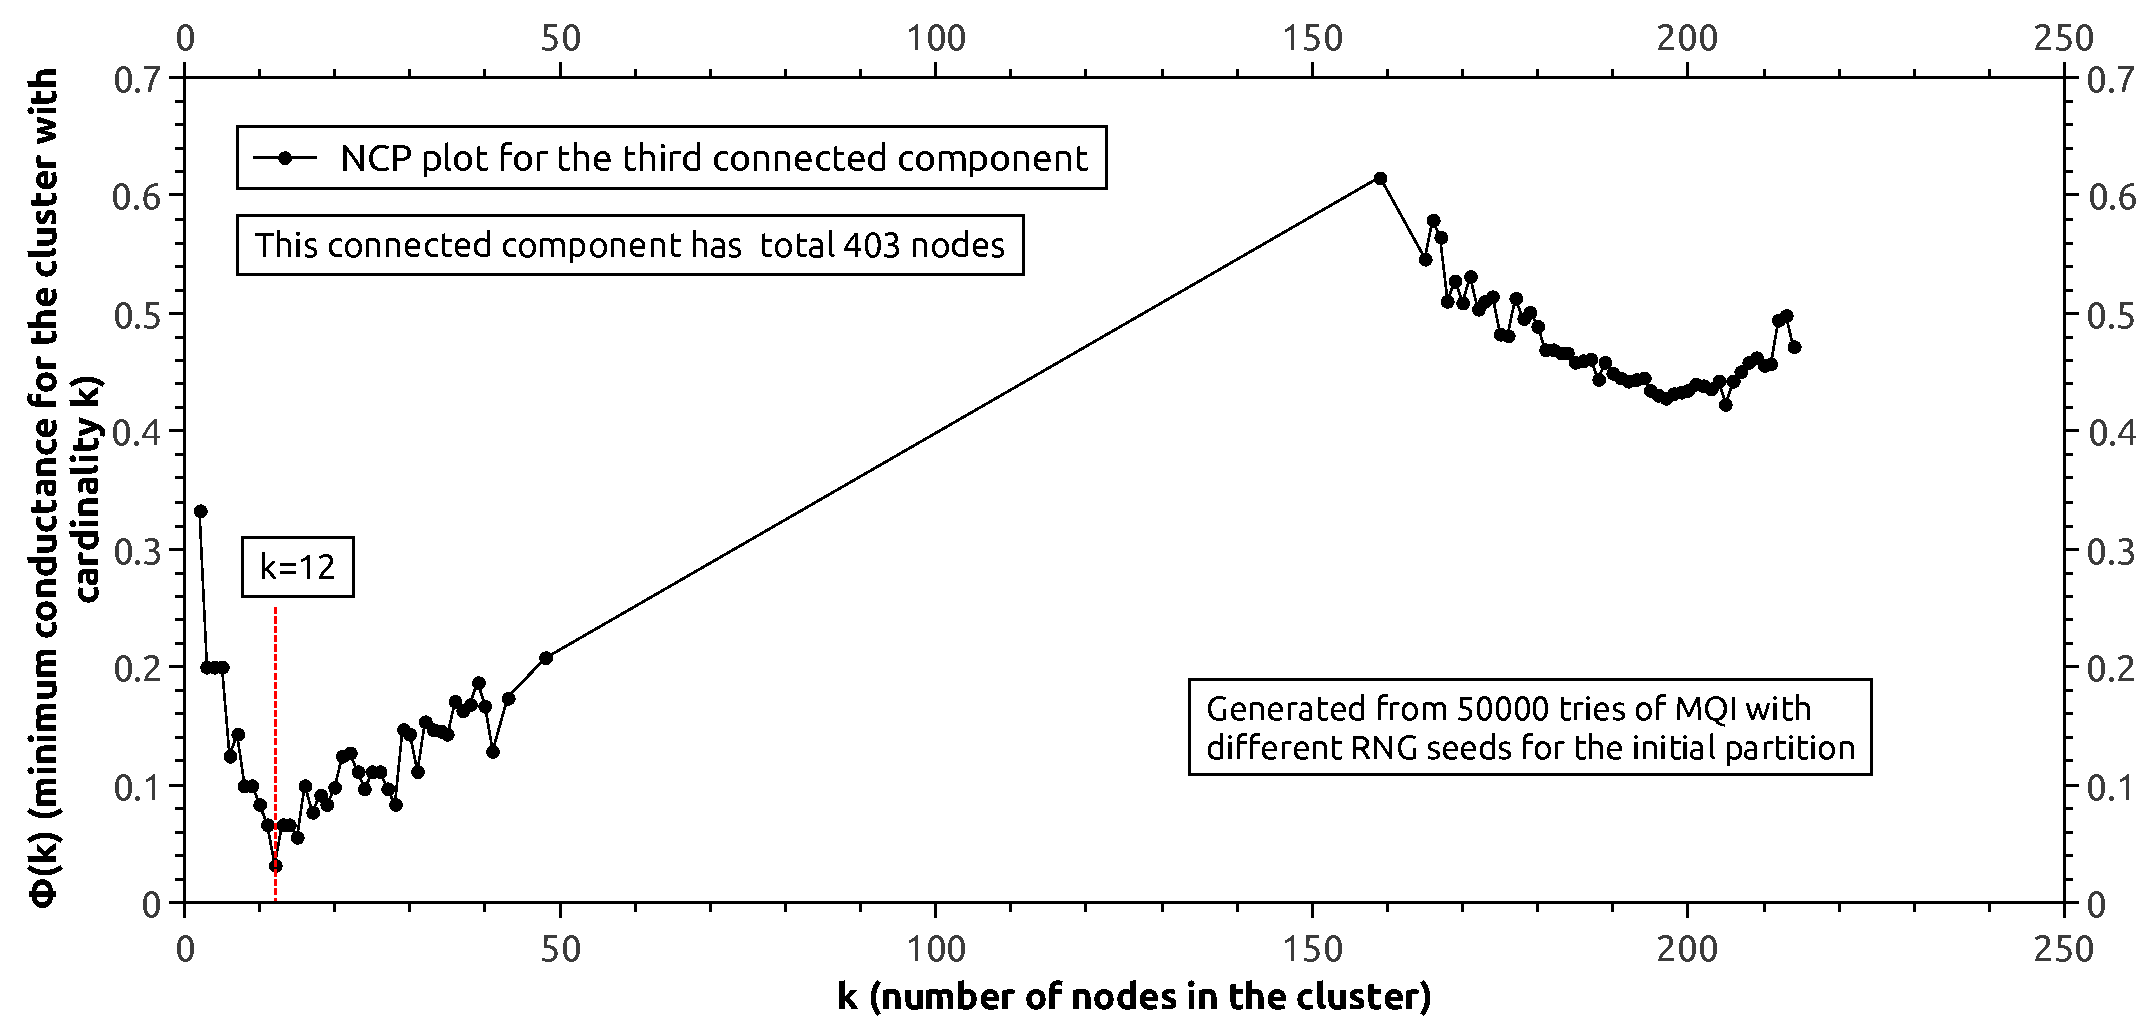
\includegraphics[scale=0.45]{MQI_3.pdf}
\caption{NCP plot of the third connected component}
\end{center}
\end{figure}
\newpage
After spectral clustering returns three connected components, with size $k=9$, $k=11$ and $k=403$, applying MQI method to each connected component, we get three NPC plots shown in Figure 5 and Figure 6. From these three figures, we can tell the first connected component's most communities-like set has size $k=4$, the second one has size $k=5$ and the third one has size $k=12$. Comparing figure 6 with figure 4, we will find not only their overall shapes are similar, but also their minima locations are very close. However, their minima have totally different meanings. One stands for possible connected component size in the original graph while the other stands for the most communities-like set size in the third component. Their overall shapes are very similar is because the sizes of other connected components are very small compared to the third component ($\frac{9}{403}\approx 2.23\%$ and $\frac{11}{403}\approx 2.73\%$). To further visualize these three components in the original graph, we plot figure 7:
\begin{figure}[H]
  \begin{subfigure}[b]{0.333\textwidth}
    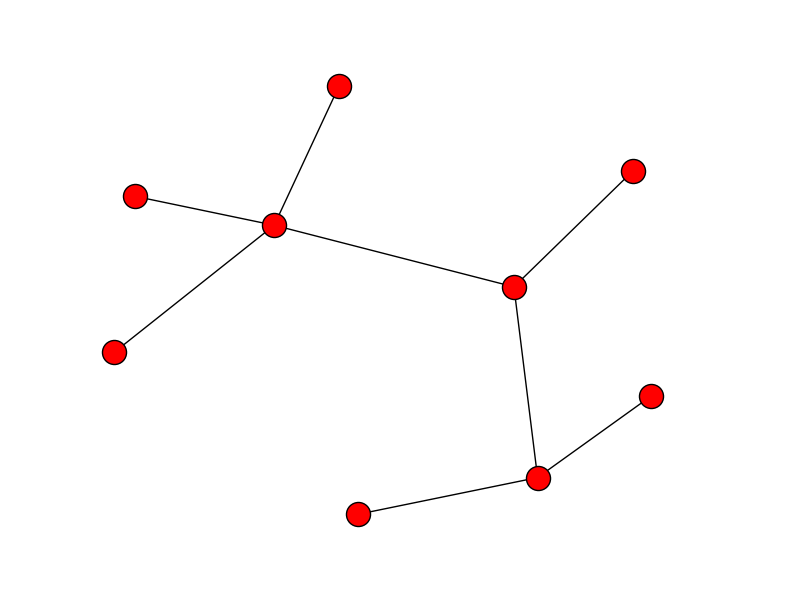
\includegraphics[scale=0.3]{cluster1.png}      
  \end{subfigure}
  \begin{subfigure}[b]{0.333\textwidth}
    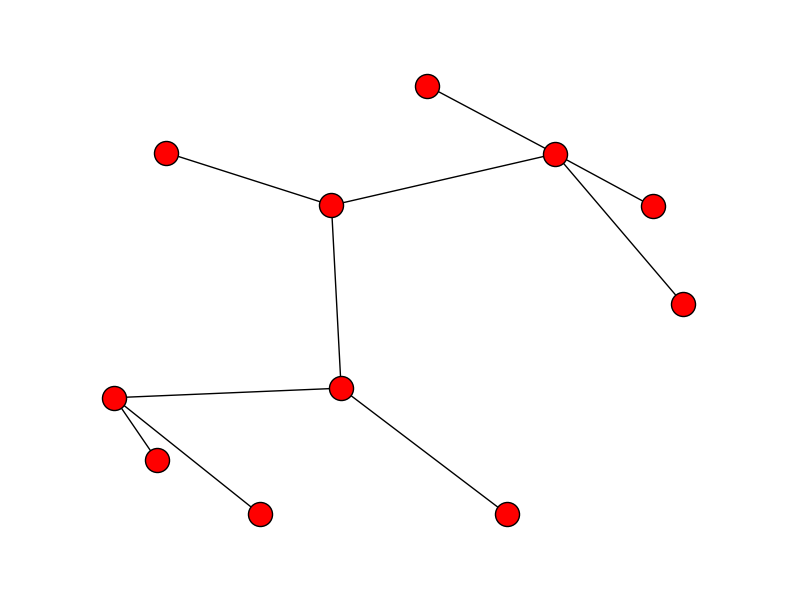
\includegraphics[scale=0.3]{cluster3.png}  
  \end{subfigure}
  \begin{subfigure}[b]{0.333\textwidth}
    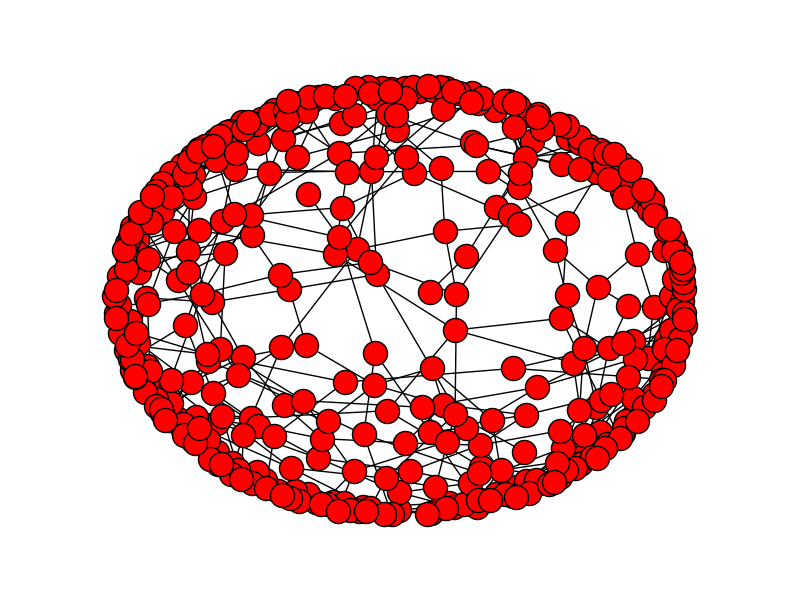
\includegraphics[scale=0.3]{cluster2.png}  
  \end{subfigure}
  \caption{three connected components in the original graph}
\end{figure}

Actually, from figure 7, we can easily tell that the most communities-like sets for the first and second components are $k=4$ and $k=5$, which totally agree with the most communities-like set sizes returned from NCP plots of these two components.
\begin{center}
{\Large \textbf{5. Conclusions}}
\end{center}
In this project, we not only learn two specific methods (techniques), spectral clustering method and max flow quotient cut improvement (MQI) method, to handle clustering problems, but also investigated statistical properties of community-like sets of nodes in complicated road network graphs, which have multiple connected components. In particular, we defined a network community profile plot (NCP plot), whose minimum will tell us the information of most communities-like sets in that graph. Also we discovered that only applying MQI method will not give us enough cluster information for this specific type graphs, while (on the contrary) combining spectral clustering method with MQI method will yield very clear and reliable cluster informations.\\\\\\
\begin{center}
{\Large \textbf{References}}
\end{center}
$[1]$. M. Momtazpour and N. Ramakrishnan, “Characterizing Taxi Flows in New York City.”\\
$[2]$. F. Bistaffa, A. Farinelli, and S. D. Ramchurn, “Sharing rides with friends: a coalition formation algorithm for ridesharing,” 2014.\\
$[3]$. M. Momtazpour, P. Butler, N. Ramakrishnan, M. S. Hossain, M. C. Bozchalui, and R. Sharma, “Charging and storage infrastructure design for electric vehicles,” ACM Trans. Intell. Syst. Technol. TIST, vol. 5, no. 3, p. 42, 2014.\\
$[4]$. Z. Cao, S. Wang, G. Forestier, A. Puissant, and C. F. Eick, “Analyzing the composition of cities using spatial clustering,” in Proceedings of the 2nd ACM SIGKDD International Workshop on Urban Computing, 2013, p. 14.\\
$[5]$. C. K. VACA RUIZ, “Spatial analysis of online data to track cities’ socio economic indicators and urban land use,” 2014.\\
$[6]$. S. Jiang, J. Ferreira Jr, and M. C. Gonzalez, “Discovering urban spatial-temporal structure from human activity patterns,” in Proceedings of the ACM SIGKDD international workshop on urban computing, 2012, pp. 95–102.\\
$[7]$. J. Leskovec, K. Lang, A. Dasgupta, M. Mahoney. Community Structure in Large Networks: Natural Cluster Sizes and the Absence of Large Well-Defined Clusters. Internet Mathematics 6(1) 29--123, 2009.\\
$[8]$. $https://snap.stanford.edu/data/\#road$.\\
$[9]$. J. Cheeger. A lower bound for the smallest eigenvalue of the laplacian. In Problems in Analysis, Papers dedicated to Salomon Bochner, pages 195–199. Princeton University Press, 1969.\\
$[10]$. W.E. Donath and A.J. Hoffman. Algorithms for partitioning graphs and computer logic based on eigenvectors of connection matrices. IBM Technical Disclosure Bulletin, 15(3):938–944, 1972.\\
$[11]$. M. Fiedler. Algebraic connectivity of graphs. Czechoslovak Mathematical Journal, 23(98):298–305, 1973.\\
$[12]$. G. Karypis and V. Kumar. A fast and high quality multilevel scheme for partitioning irregular graphs. SIAM Journal on Scientific Computing, 20:359–392, 1998.\\
$[13]$. K. Lang and S. Rao. A flow-based method for improving the expansion or conductance of graph cuts. In IPCO ’04: Proceedings of the 10th International IPCO Conference on Integer Programming and Combinatorial Optimization, pages 325–337, 2004.\\
$[14]$. R. Kannan, S. Vempala, and A. Vetta. On clusterings: Good, bad and spectral. Journal of the ACM, 51(3):497–515, 2004.\\
$[15]$. G.W. Flake, R.E. Tarjan, and K.Tsioutsiouliklis. Graph clustering and minimum cut trees. Internet Mathematics, 1(4):385–408, 2003.\\
$[16]$. G.W. Flake, S. Lawrence, and C.L. Giles. Efficient identification of web communities. In KDD ’00: Proceedings of the 6th ACM SIGKDD International Conference on Knowledge Discovery and Data Mining, pages 150–160, 2000.\\
$[17]$. G.W. Flake, S. Lawrence, C.L. Giles, and F.M. Coetzee. Self-organization and identification of web communities. Computer, 35(3):66–71, 2002.\\
$[18]$. F. Radicchi, C. Castellano, F. Cecconi, V. Loreto, and D. Parisi. Defining and identifying communities in networks. Proceedings of the National Academy of Sciences of the United States of America, 101(9):2658–2663, 2004.\\
$[19]$. U. von Luxburg, A tutorial on spectral clustering, Tech. Rep. 149, Max Planck Institute for Biological Cybernetics, August 2006.
$[20]$. K. Lang and S. Rao. A flow-based method for improving the expansion or conductance of graph cuts. In IPCO ’04: Proceedings of the 10th International IPCO Conference on Integer Programming and Combinatorial Optimization, pages 325–337, 2004.
\end{document}